\documentclass[../main/report.tex]{subfiles}
\begin{document}

\section{Troubleshooting and workarounds}

After testing it became apparent there was two major issues that needed to be fixed with the PCB.
Firstly the pin on the FPGA reserved for the clock could not be used for a clock.
Secondly the clock itself had been wired up wrongly.

\subsection*{FPGA clock pin problem}
When the code for the FPGA was tested with the pins from the PCB, an error occured.
The FPGA demanded a special pin for the clock, but the PCB routed the clock into a regular GPIO pin.
After a checkup a pin on the EBI bus was shown to be able to work as clock for the FPGA.
The clock is connected by jumpers to the FPGA, so the pin on the EBI bus and the clock pin on the FPGA was changed around with wires.

\subsection*{Wrongly wiring of clock}

When wiring the clock up a poorly designed data sheet for the clock component caused so much confusion that the wiring itself was wrong on the PCB, see figure \ref{fig:pcb-clock}.

\begin{figure}[H]
    \centering
    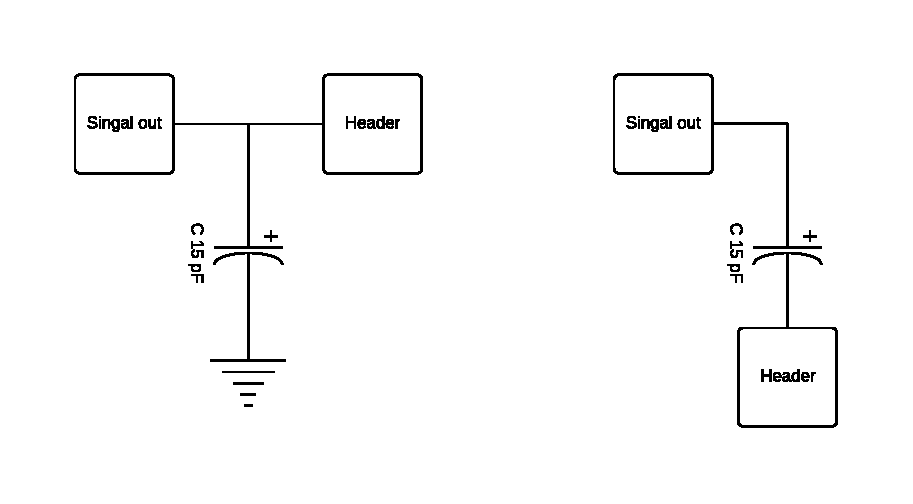
\includegraphics[width=0.65\textwidth]{../pcb/assets/pcb-clock.pdf}
    \label{fig:pcb-clock}
    \caption{On the left: How the clock from the FPGA is suppose to be connected.
             On the right: how it got connected on the PCB.}
\end{figure}

This caused the clock not to function at all, and with it the rest of the system.
Our solution to this problem is to solder together the place where the first capacitor was to make room for the signal to flow freely to the header.
Afterwards a thru-hole version of the same capacitor was placed on one of the soldering pads and the other end grounded.
This caused the circuit on the board to fully match up with the correct circuit from the data sheet.

\end{document}
